\documentclass[tikz,border=0pt]{standalone}
\usepackage[T1]{fontenc}
\usepackage{helvet}
\usepackage{textcomp}
\renewcommand{\familydefault}{\sfdefault}
\usetikzlibrary{arrows.meta,calc}
\definecolor{ink}{HTML}{252525}
\definecolor{linegray}{HTML}{747474}
\definecolor{receiving}{HTML}{D55E00}
\definecolor{mirror}{HTML}{0072B2}
\definecolor{fat}{HTML}{F5E8BC}
\definecolor{muscle}{HTML}{F3E4E0}
\begin{document}
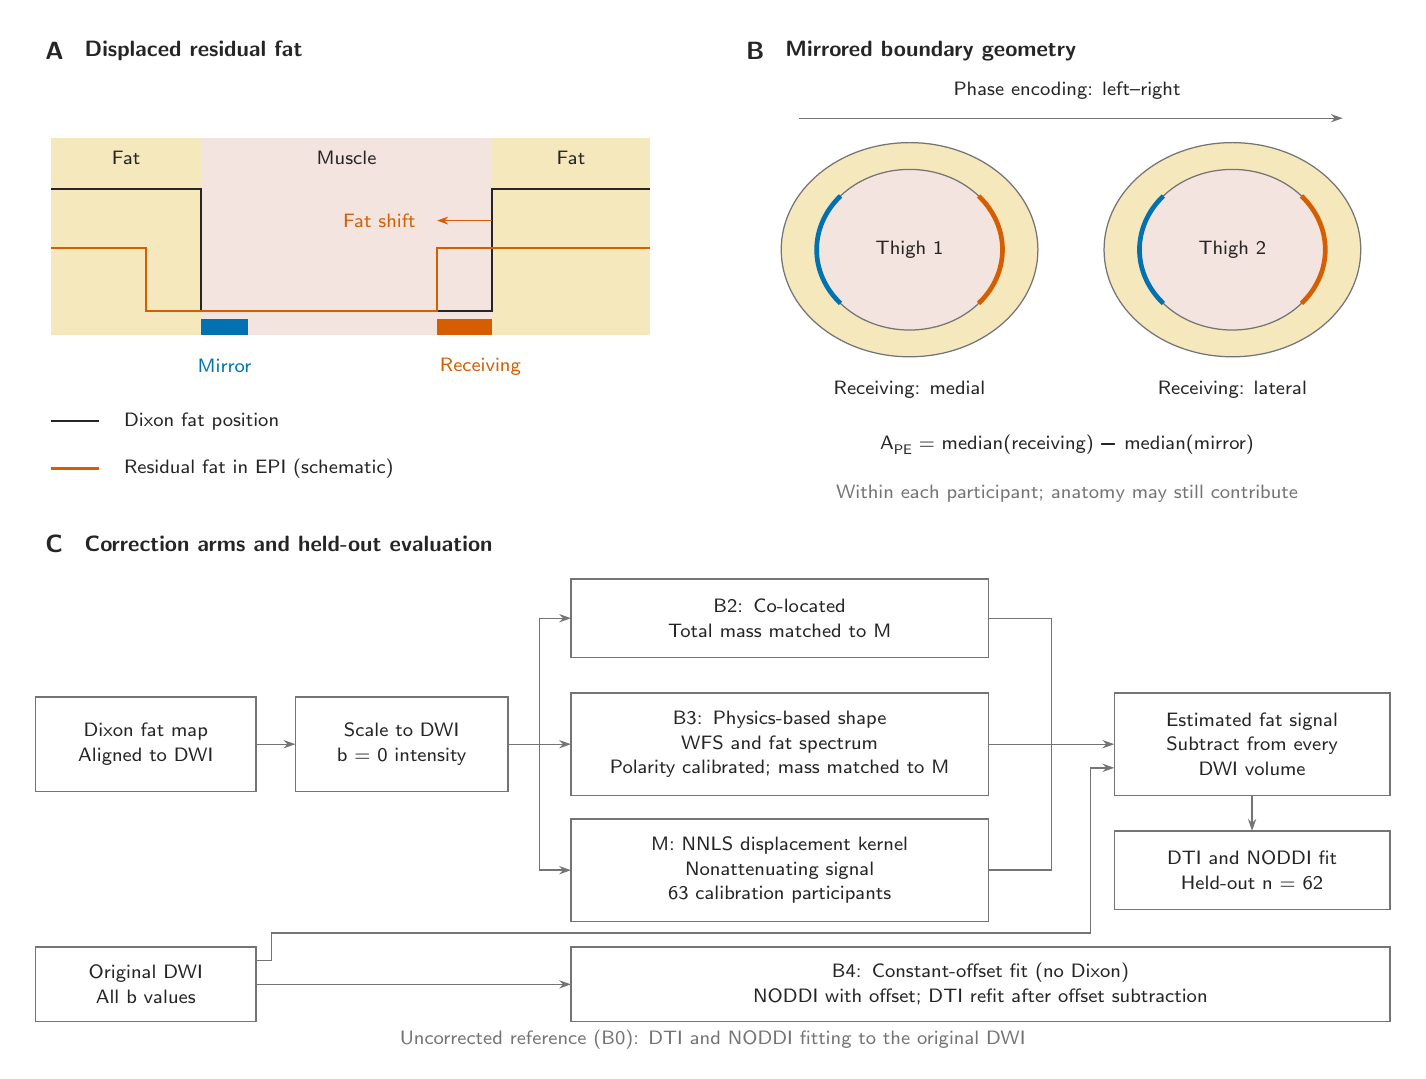
\begin{tikzpicture}[x=1mm,y=1mm,text=ink,
  font=\sffamily\fontsize{7.5}{9}\selectfont,
  box/.style={draw=linegray,line width=.5pt,fill=white,align=center,
    inner xsep=1.2mm,inner ysep=1mm,outer sep=0pt},
  flow/.style={-{Stealth[length=1.5mm,width=1.05mm]},draw=linegray,line width=.5pt},
  branch/.style={draw=linegray,line width=.5pt},
  panel/.style={anchor=west,font=\sffamily\bfseries\fontsize{9.5}{10}\selectfont},
  heading/.style={anchor=west,font=\sffamily\bfseries\fontsize{8.5}{10}\selectfont}]
\path[use as bounding box] (0,0) rectangle (174,130);
\node[panel] at (1,127) {A};
\node[heading] at (6,127) {Displaced residual fat};
\node[panel] at (90,127) {B};
\node[heading] at (95,127) {Mirrored boundary geometry};

\fill[fat] (3,91) rectangle (22,116);
\fill[muscle] (22,91) rectangle (59,116);
\fill[fat] (59,91) rectangle (79,116);
\node at (12.5,113.5) {Fat};
\node at (40.5,113.5) {Muscle};
\node at (69,113.5) {Fat};
\draw[ink,line width=.7pt] (3,109.5) -- (22,109.5) -- (22,94) -- (59,94) -- (59,109.5) -- (79,109.5);
\draw[receiving,line width=.85pt] (3,102) -- (15,102) -- (15,94) -- (52,94) -- (52,102) -- (79,102);
\fill[mirror] (22,91) rectangle (28,93);
\fill[receiving] (52,91) rectangle (59,93);
\draw[-{Stealth[length=1.4mm,width=1mm]},receiving,line width=.65pt] (59,105.5) -- (52,105.5);
\node[text=receiving,anchor=east] at (50.5,105.5) {Fat shift};
\node[text=mirror] at (25,87) {Mirror};
\node[text=receiving] at (57.5,87) {Receiving};
\draw[ink,line width=.7pt] (3,80) -- (9,80);
\node[anchor=west] at (11,80) {Dixon fat position};
\draw[receiving,line width=.85pt] (3,74) -- (9,74);
\node[anchor=west] at (11,74) {Residual fat in EPI (schematic)};

\node at (132,122) {Phase encoding: left--right};
\draw[flow] (98,118.5) -- (167,118.5);
\foreach \x/\name in {112/1,153/2}{
  \filldraw[fill=fat,draw=linegray,line width=.45pt] (\x,101.8) ellipse[x radius=16.3mm,y radius=13.6mm];
  \filldraw[fill=muscle,draw=linegray,line width=.45pt] (\x,101.8) ellipse[x radius=11.8mm,y radius=10.2mm];
  \draw[receiving,line width=1.7pt] ({\x+11.8*cos(-42)},{101.8+10.2*sin(-42)}) arc[start angle=-42,end angle=42,x radius=11.8mm,y radius=10.2mm];
  \draw[mirror,line width=1.7pt] ({\x+11.8*cos(138)},{101.8+10.2*sin(138)}) arc[start angle=138,end angle=222,x radius=11.8mm,y radius=10.2mm];
  \node at (\x,101.8) {Thigh \name};
}
\node at (112,84) {Receiving: medial};
\node at (153,84) {Receiving: lateral};
\node at (132,77) {A\raisebox{-0.5ex}{\fontsize{5.25}{6}\selectfont PE} = median(receiving) \textminus\ median(mirror)};
\node[text=linegray] at (132,70.8) {Within each participant; anatomy may still contribute};

\node[panel] at (1,64.5) {C};
\node[heading] at (6,64.5) {Correction arms and held-out evaluation};
\node[box,text width=25.6mm,minimum height=12mm] (dixon) at (15,39)
  {Dixon fat map\\Aligned to DWI};
\node[box,text width=24.6mm,minimum height=12mm] (scaled) at (47.5,39)
  {Scale to DWI\\b = 0 intensity};
\node[box,text width=50.6mm,minimum height=10mm] (b2) at (95.5,55)
  {B2: Co-located\\Total mass matched to M};
\node[box,text width=50.6mm,minimum height=13mm] (b3) at (95.5,39)
  {B3: Physics-based shape\\WFS and fat spectrum\\Polarity calibrated; mass matched to M};
\node[box,text width=50.6mm,minimum height=13mm] (kernel) at (95.5,23)
  {M: NNLS displacement kernel\\Nonattenuating signal\\63 calibration participants};
\node[box,text width=32.6mm,minimum height=13mm] (subtract) at (155.5,39)
  {Estimated fat signal\\Subtract from every\\DWI volume};
\node[box,text width=32.6mm,minimum height=10mm] (fit) at (155.5,23)
  {DTI and NODDI fit\\Held-out n = 62};
\draw[flow] (dixon.east) -- (scaled.west);
\draw[branch] (scaled.east) -- (65,39);
\draw[flow] (65,39) |- (b2.west);
\draw[flow] (65,39) -- (b3.west);
\draw[flow] (65,39) |- (kernel.west);
\draw[branch] (b2.east) -- (130,55) -- (130,39);
\draw[branch] (kernel.east) -- (130,23) -- (130,39);
\draw[flow] (b3.east) -- (subtract.west);
\draw[flow] (subtract.south) -- (fit.north);

\node[box,text width=25.6mm,minimum height=9.5mm] (original) at (15,8.5)
  {Original DWI\\All b values};
\node[box,text width=101.6mm,minimum height=9.5mm] (offset) at (121,8.5)
  {B4: Constant-offset fit (no Dixon)\\NODDI with offset; DTI refit after offset subtraction};
\draw[flow] (original.east) -- (offset.west);
\draw[flow] (29,11.5) -- (31,11.5) -- (31,15) -- (135,15) -- (135,36) -- (138,36);
\node[text=linegray,font=\sffamily\fontsize{7.5}{9}\selectfont] at (87,1.5)
  {Uncorrected reference (B0): DTI and NODDI fitting to the original DWI};
\end{tikzpicture}
\end{document}
